% Chương 3

\chapter{CHƯƠNG TRÌNH THỰC NGHIỆM} 

\label{Chapter3} 

\section{Bộ dữ liệu}

Bộ dữ liệu hình ảnh được lấy từ: \href{https://www.kaggle.com/datasets/spandanpatnaik09/face-mask-detectormask-not-mask-incorrect-mask}{Kaggle} 

*** Dữ liệu mask và Dữ liệu cảm xúc (emotion)

\begin{figure}[h!] 
	\begin{tabular}{cc}
		\centering
		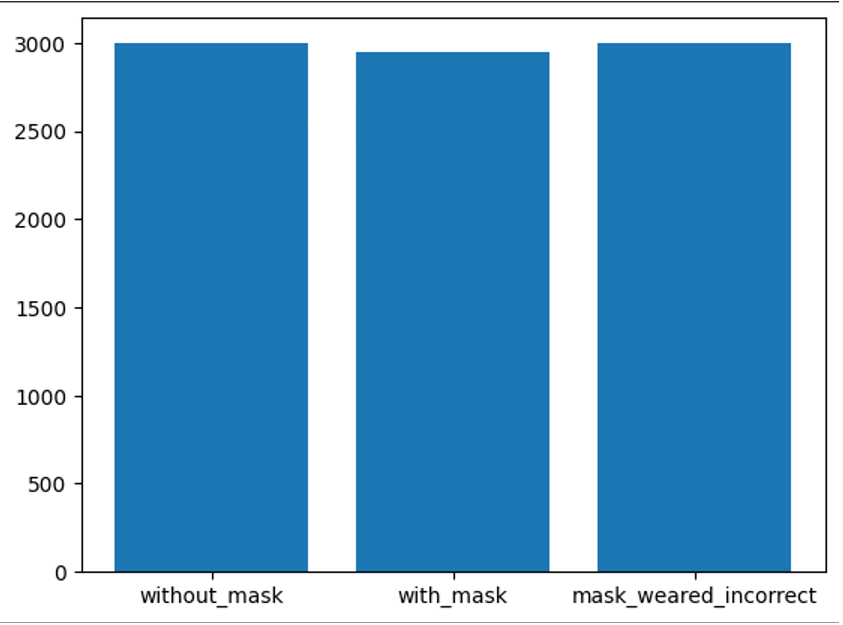
\includegraphics[width=0.5\textwidth]{mask.png} &
		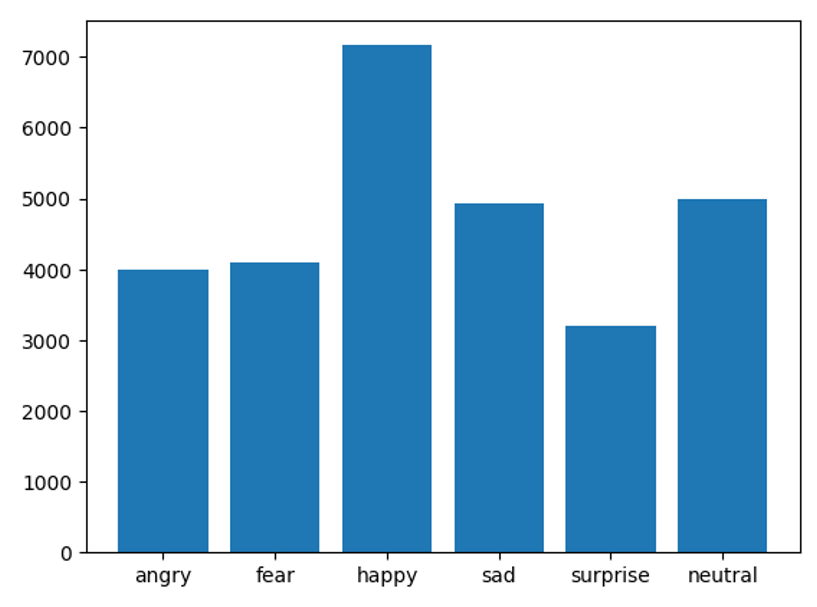
\includegraphics[width=0.5\textwidth]{emotion.png} 
	\end{tabular}
	\caption[Bộ dữ liệu mask và emotion.]{Bộ dữ liệu mask và emotion.}
	\label{fig:maskemotion}
\end{figure}

\section{Chỉ số đánh giá hiệu suất}

Để đánh giá phân loại ảnh được chính xác, các mô hình trong phần trước sữ được chạy bằng cách sử dụng bộ dữ liệu dưới dạng hình ảnh, vì vậy cần có sự điều chỉnh để nâng cấp độ chính xác của chúng. Đối với mỗi mô hình 3 kết quả điển hình được hiển thị trong CNN là:

\begin{itemize}
	\item Đồ thị độ chính xác (model ACC): ACC cho biết sự thay đổi độ chính xác của mô hình qua các vòng lặp/epochs trong quá trình huấn luyện.
	
	\item Đồ thị loss (model loss): Đồ thị loss biểu thị sự thay đổi của hàm loss của mô hình qua các vòng lặp hoặc epochs trong quá trình huấn luyện. Hàm loss tính toán sự sai khác giữa giá trị dự đoán của mô hình và giá trị thực tế.
	
	\item Confusion matrix: Về cơ bản, Confusion matrix thể hiện có bao nhiêu điểm dữ liệu thực sự thuộc vào một class, và được dự đoán là rơi vào một class. 
	
	\begin{figure}[h!]
		\centering
		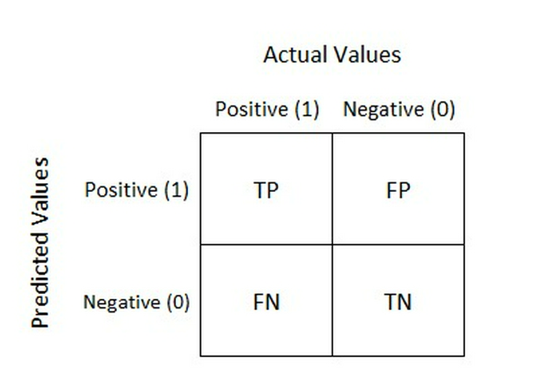
\includegraphics[width=0.7\textwidth]{cofusion.png}
		\caption[Confusion matrix.]{Confusion matrix.}
		\label{fig:cm} 
	\end{figure}

	\begin{itemize}
		\item TP (True Positive): Số lượng dự đoán chính xác.
		
		\item TN (True Negative): Số lương dự đoán chính xác một cách gián tiếp. Là khi mô hình dự đoán đúng một người không bị bệnh tức là việc không chọn trường hợp bị bệnh là chính xác.
		
		\item FP (False Positive - Type 1 Error): Số lượng các dự đoán sai lệch. Là khi mô hình dự đoán một người bị bệnh và người đó hoàn toàn khỏe mạnh.
		
		\item FN (False Negative - Type 2 Error): Số lượng các dự đoán sai lệch một cách gián tiếp. Là khi mô hình dự đoán một người không bị bệnh nhưng người đó bị bệnh, tức là việc không chọn trường hợp bị bệnh là sai. 		
	\end{itemize}
	$\Longrightarrow$ Từ 4 chỉ số TP, TN, FP, FN, ta có 4 chỉ số để đánh giá mức độ tin cậy của một mô hình:
\end{itemize}

\begin{itemize}
	\item Accuracy: Được tính bằng cách chia tổng số dự đoán đúng cho tất cả các dự đoán.
	
	\begin{figure}[h!]
		\centering
		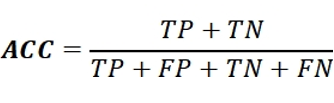
\includegraphics[width=0.45\textwidth]{acc1.png}
		\caption[Accuracy.]{Accuracy.}
		\label{fig:acc} 
	\end{figure}
		
	\item Precision: Trong tất cả các dự đoán Positive được đưa ra, bao nhiêu dự đoán là chính xác.
	
	\begin{figure}[h!]
		\centering
		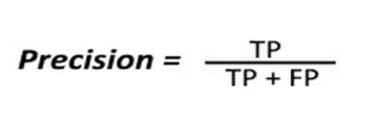
\includegraphics[width=0.6\textwidth]{precision.png}
		\caption[Precision.]{Precision.}
		\label{fig:precision} 
	\end{figure}
	
	\item Recall: Trong tất cả các trường hợp Positive, bao nhiêu trường hợp đã được dự đoán chính xác.		
	
	\begin{figure}[h!]
		\centering
		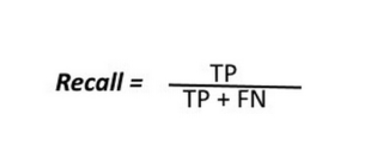
\includegraphics[width=0.6\textwidth]{recall.png}
		\caption[Recall.]{Recall.}
		\label{fig:recall} 
	\end{figure}

	\item F1-Score: Dùng để đánh giá mức độ tin cậy chung của mô hình
	
	\begin{figure}[h!]
		\centering
		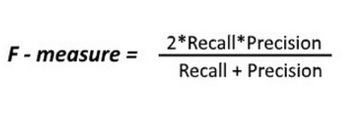
\includegraphics[width=0.6\textwidth]{score.png}
		\caption[F1-Score.]{F1-Score.}
		\label{fig:score} 
	\end{figure}
\end{itemize}

\section{Huấn luyện mô hình và kết quả thực nghiệm}

Do các bước tiền xử lý dữ liệu của 2 mô hình là như nhau thế nên trong báo cáo này em chỉ trình bày cách nhóm em xử lý dữ liệu của bộ dự hiệu khẩu trang.

\subsection{Tiền xử lý dữ liệu} 

*** Import một số thư viện để xử lí và phân tích trực quan dữ liệu:

\begin{lstlisting}[style=codePython]
  	import glob
  	import shutil
  	import cv2 
  	from PIL import Image
  	import PIL
  	import os
  	import numpy as np
  	import pandas as pd
  	import matplotlib.pyplot as plt
  	import seaborn as sns
  	import random 
  	from sklearn.model_selection import train_test_split
  	import tensorflow as tf
  	import keras
  	from keras.preprocessing import image
  	from keras.models import Sequential
  	from keras.layers import Conv2D, MaxPool2D, Flatten,Dense,Dropout,BatchNormalization
  	from keras import regularizers

  	import warnings
  	# Ignore waring
  	warnings.filterwarnings('ignore')  	
\end{lstlisting}

*** Tiền xử lý dữ liệu: 

\begin{itemize}
	\item Tiền xử lý dữ liệu là một bước rất quan trọng trong việc giải quyết bất kỳ vấn đề nào trong lĩnh vực học máy. Hầu hết các bộ dữ liệu được sử dụng trong các vấn đề liên quan đến học máy cần được xử lý, làm sạch và biến đổi trước khi một thuật toán có thể được huấn luyện trên những bộ dữ liệu này.
	
	\item Load dữ liệu hình ảnh vào tập train và labels.
	
	\begin{itemize}
		\item Tạo đường dẫn:
		
		\begin{lstlisting}[style=codePython]
			mask_path = ['/without_mask/*','/with_mask/*','/incorrect_mask/*' ]
			
			train_path = '/content/drive/MyDrive/Dataset/processed'			
		\end{lstlisting}
		
		\item Load dữ liệu:
		
		\begin{lstlisting}[style=codePython]
			X = []
			y = []
			for i, path in enumerate(mask_path):
			for name in glob.glob(train_path + path):
			img = cv2.imread(name)
			img = cv2.cvtColor(img,cv2.COLOR_BGR2RGB)
			img = cv2.resize(img,(48,48))
			X.append((img))
			y.append(i)
			len(X)					
		\end{lstlisting}
	
		\item Chuẩn hóa dữ liệu hình ảnh: Các giá trị pixel được đưa về các giá trị trong khoảng từ 0 đến 1 giúp mô hình học tốt hơn.
		
		\begin{lstlisting}[style=codePython]
			X = np.array(X)/255.
			y = np.array(y)			
		\end{lstlisting}
	
		\item Phân tích dữ liệu thành tập train và tập test: Sau đó ta tạo 4 biến, gồm X$\_$train, y$\_$train và X$\_$test, y$\_$test. Với đối số truyền vào là giá trị X, y ta đã lấy từ dữ liệu bên trên, test$\_$size trả về cho ta phần trăm dữ liệu được chia, ví dụ 0.2 tương ứng với dữ liệu được chia thành 20\% giá trị là test, còn lại là dữ liệu train. random$\_$state bằng một số tương ứng nào đó để đảm bảo mỗi lần ta chạy lại mô hình, giá trị phân tách ngẫu nhiên nhận được là giống nhau, bạn có thể cho số nào bất kỳ. 
		
		 \begin{lstlisting}[style=codePython]
		 	X_train, X_test, y_train, y_test = train_test_split(X, y, test_size=0.2, random_state=2)			
		 \end{lstlisting}
	 
	 	\item Chuẩn hóa dữ liệu output: Chuyển về dạng onehot để phân biệt nhiều ảnh một cách dễ dàng  
	 	
	 	\begin{lstlisting}[style=codePython]
	 		from sklearn.preprocessing import OneHotEncoder
	 		encoder = OneHotEncoder()
	 		encoder.fit(y_train.reshape(-1,1))
	 		y_train = encoder.transform(y_train.reshape(-1,1)).toarray()
	 		y_test = encoder.transform(y_test.reshape(-1,1)).toarray()
	 		print(y_train) 				
	 	\end{lstlisting}		
	\end{itemize}
\end{itemize} 

\subsection{Mô hình huấn luyện CNN}

\subsubsection{Mô hình nhận dạng khẩu trang}

\begin{lstlisting}[style=codePython]
	inp = Input(shape = (48,48,3))
	cnn = Conv2D(filters =16,kernel_size = 3,activation ='relu')(inp)
	pooling = MaxPooling2D(pool_size =(2,2))(cnn)
	drop = Dropout(0.2)(pooling)
	
	cnn = Conv2D(filters =32,kernel_size = 3,activation ='relu')(inp)
	pooling = MaxPooling2D(pool_size =(2,2))(cnn)
	drop = Dropout(0.2)(pooling)
	
	cnn = Conv2D(filters =64,kernel_size = 4,activation ='relu')(inp)
	pooling = MaxPooling2D(pool_size =(2,2))(cnn)
	drop = Dropout(0.2)(pooling)
	
	cnn = Conv2D(filters =128, kernel_size =4,activation ='relu')(drop)
	pooling = MaxPooling2D(pool_size =(2,2))(cnn)
	drop = Dropout(0.2)(pooling)
	
	f =Flatten()(pooling)
	
	fc1 = Dense(units =128, activation ='relu')(f)
	fc2 = Dense(units =64, activation ='relu')(fc1)
	fc3 = Dense(units =32, activation ='relu')(fc2)
	out = Dense(units =3, activation ='softmax')(fc3)
	
	model =Model(inputs = inp,outputs =out)
	model.summary()	 				
\end{lstlisting}

$\Longrightarrow$ Đoạn code này định nghĩa một mô hình mạng neural tích chập (CNN) để phân loại ảnh với ba lớp đầu ra. 

\begin{itemize}
	\item Biến inp định nghĩa một hình dạng đầu vào là 48x48 pixel với 3 kênh màu (RGB).
	
	\item Sau đó là 4 lớp tích chập (Conv2D) với số lượng bộ lọc, kích thước kernel và kích hoạt ReLU tăng dần. Lớp đệm padding để giữ nguyên kích thưởng đầu ra. Mỗi lớp tích chập được theo sau bởi một lớp giảm kích thước (MaxPooling2D) để giảm kích thước không gian của đầu ra từ lớp tích chập. Các lớp giảm kích thước này giúp giảm thiểu quá khớp và cải thiện tốc độ và hiệu suất. Mỗi lớp giảm kích thước cũng được theo sau bởi một lớp dropout (Dropout) với tỷ lệ 0.2, loại bỏ ngẫu nhiên 20\% của các neuron để giảm thiểu quá khớp.
	
	\item Sau các lớp tích chập và giảm kích thước, đầu ra đã được làm phẳng từ lớp giảm kích thước cuối cùng, được đưa vào ba lớp kết nối đầy đủ (Dense) với số lượng đơn vị giảm dần và kích hoạt ReLU. Lớp đầu ra có 3 đơn vị với hàm kích hoạt softmax, xuất ra xác suất lớp cho mỗi ảnh đầu vào.
	
	\item Mô hình được tạo ra bằng cách sử dụng hàm Model từ Keras, với lớp đầu vào và đầu ra được xác định là inp và out, tương ứng.
	
	\item Cuối cùng, hàm model.summary() được sử dụng để in ra tóm tắt kiến trúc mô hình, bao gồm các loại lớp, hình dạng và số lượng tham số.
\end{itemize}

*** Sau khi đã xây dựng được kiến trúc của mô hình . Bước tiếp theo là thực hiện huấn luyện mô hình: 

\begin{lstlisting}[style=codePython]
	optimizer1 = tensorflow.keras.optimizers.Adam(learning_rate = 0.0001)
	model.compile(optimizer = optimizer1, loss = 'categorical_crossentropy',metrics =['accuracy'])
	
	history = model.fit(X_train,y_train,batch_size =16, epochs =25,validation_data =(X_test,y_test))				
\end{lstlisting}

\subsubsection{Mô hình nhận dạng cảm xúc}

\begin{lstlisting}[style=codePython]
	model= tf.keras.models.Sequential()
	model.add(Conv2D(32, kernel_size=(3, 3), padding='same', activation='relu', input_shape=(48, 48,1)))
	model.add(Conv2D(64,(3,3), padding='same', activation='relu' ))
	model.add(BatchNormalization())
	model.add(MaxPool2D(pool_size=(2, 2)))
	model.add(Dropout(0.25))
	
	model.add(Conv2D(128,(5,5), padding='same', activation='relu'))
	model.add(BatchNormalization())
	model.add(MaxPool2D(pool_size=(2, 2)))
	model.add(Dropout(0.25))
	
	model.add(Conv2D(512,(3,3), padding='same', activation='relu', kernel_regularizer=regularizers.l2(0.01)))
	model.add(BatchNormalization())
	model.add(MaxPool2D(pool_size=(2, 2)))
	model.add(Dropout(0.25))
	
	model.add(Conv2D(512,(3,3), padding='same', activation='relu', kernel_regularizer=regularizers.l2(0.01)))
	model.add(BatchNormalization())
	model.add(MaxPool2D(pool_size=(2, 2)))
	model.add(Dropout(0.25))
	
	model.add(Flatten()) 
	model.add(Dense(256,activation = 'relu'))
	model.add(BatchNormalization())
	model.add(Dropout(0.25))
	
	model.add(Dense(512,activation = 'relu'))
	model.add(BatchNormalization())
	model.add(Dropout(0.25))
	
	model.add(Dense(6, activation='softmax'))
	model.summary()					
\end{lstlisting}

$\Longrightarrow$ Đây là một mô hình CNN (Convolutional Neural Network) có kiến trúc phức tạp. Mô hình bao gồm 5 lớp tích chập (Conv2D) với các bộ lọc kích thước khác nhau và hàm kích hoạt là ReLU.

\begin{itemize}
	\item Lớp đầu tiên có 32 bộ lọc kích thước 3x3, lớp thứ hai có 64 bộ lọc kích thước kernel 3x3, lớp thứ ba là lớp có 128 bộ lọc  kích thước 5x5 và lớp cuối cùng là 2 lớp với 512 bộ lọc kích thước 3x3 và kết hợp với hàm chính quy (regularization) để giúp mô hình tránh overfitting.
	
	\item Sau mỗi lớp tích chập, model sử dụng một lớp BatchNormalization để chuẩn hóa giá trị và tăng tốc độ hội tụ. Lớp MaxPool2D được sử dụng để giảm kích thước của đầu ra và giảm số lượng tham số của mô hình. Lớp Dropout được sử dụng để giảm hiện tượng overfitting.
	
	\item Cuối cùng, một lớp Dense với 256 đơn vị và hàm kích hoạt ReLU được thêm vào mô hình, sau đó theo sau bởi một lớp Dropout và BatchNormalization. Sau đó, một lớp Dense với 512 đơn vị và hàm kích hoạt ReLU được chỉ định kế tiếp và kết thúc bằng lớp Dense với 6 đơn vị đầu ra với hàm kích hoạt soft$\_$max (6 lớp tương ứng với 6 cảm xúc).
	\item Mô hình được tạo ra bằng cách sử dụng hàm Model từ Keras, với lớp đầu vào và đầu ra được xác định là inp và out, tương ứng.
	
	\item Cuối cùng, hàm model.summary() được sử dụng để in ra tóm tắt kiến trúc mô hình, bao gồm các loại lớp, hình dạng và số lượng tham số.
\end{itemize}

*** Sau khi đã xây dựng được kiến trúc của mô hình . Bước tiếp theo là thực hiện huấn luyện mô hình: 

\begin{lstlisting}[style=codePython]
	learning_rate = 0.0001
	optimizer1 = tf.keras.optimizers.Adam(learning_rate = 0.0001)
	
	model.compile(optimizer = optimizer1, loss = 'categorical_crossentropy',metrics =['accuracy'])
	
	history = model.fit(X_train, y_train, epochs=40,validation_data=(X_test_scaled, y_test),batch_size = 64,shuffle = True)					
\end{lstlisting}

*** Từ bước huấn luyện mô hình, ta có: 

\begin{itemize}
	\item optimizer1: Optimizer được khởi tạo bằng cách sử dụng Adam optimizer từ tensorflow.keras.optimizers, với learning$\_$rate = 0.0001
	
	\item model.compile(): Cấu hình mô hình với optimizer, hàm mất mát là categotical$\_$crossentropy và các metric là accuracy để đánh giá hiệu suất mô hình.
	
	\item model.fit(): Huấn luyện mô hình trên dữ liệu huấn luyện (X$\_$train, y$\_$train) với các tham số như batch$\_$size, epochs, và sử dụng dữ liệu kiểm tra (X$\_$test, y$\_$test) để đánh giá hiệu suất của mô hình trong quá trình huấn luyện.
\end{itemize}

\subsection{Tiêu chí ảnh hưởng đến mô hình}	

Có nhiều yếu tố ảnh hưởng đến độ hiệu quả của một mô hình máy học. Dưới đây là một số tiêu chí quan trọng:

\begin{itemize}
	\item Độ rõ ràng và độ phong phú của dữ liệu: Mô hình sẽ hoạt động tốt hơn khi dữ liệu huấn luyện rõ ràng, có độ phân loại cao và đủ đa dạng. Dữ liệu không rõ ràng, nhiễu và thiếu thông tin có thể làm giảm độ hiệu quả của mô hình.
	
	\item Số lượng và chất lượng dữ liệu: Một số lượng dữ liệu huấn luyện đủ lớn có thể giúp mô hình học được các mẫu và mối quan hệ phức tạp. Đồng thời, chất lượng dữ liệu cũng quan trọng, bao gồm độ chính xác, đồng nhất và đại diện cho phân phối dữ liệu thực tế.
	
	\item Chọn mô hình phù hợp: Một mô hình phải được lựa chọn dựa trên yêu cầu cụ thể của bài toán. Mô hình phải có khả năng học và biểu diễn các mẫu và quan hệ trong dữ liệu một cách hiệu quả.
	
	\item Quá trình huấn luyện: Thời gian huấn luyện, tỷ lệ học tập, thuật toán tối ưu hóa và các siêu tham số khác cũng có thể ảnh hưởng đến hiệu quả của mô hình. Quá trình huấn luyện phải được điều chỉnh và tối ưu để đạt được kết quả tốt.
	
	\item Tính diễn giải và khả năng áp dụng: Một mô hình có khả năng diễn giải tốt và có thể áp dụng vào thực tế sẽ có hiệu quả cao hơn. Sự diễn giải giúp người dùng hiểu rõ quyết định của mô hình và tin tưởng vào kết quả dự đoán.	
\end{itemize}

\subsection{Tiêu chí đánh giá mô hình}

Khi đánh giá huấn luyện một mô hình máy học, có một số tiêu chí quan trọng cần xem xét. Dưới đây là một số tiêu chí phổ biến để đánh giá mô hình:

\begin{itemize}
	\item Độ chính xác (Accuracy): Đây là tiêu chí cơ bản để đánh giá khả năng dự đoán chính xác của mô hình trên tập dữ liệu kiểm tra. Độ chính xác được tính bằng tỷ lệ giữa số lượng dự đoán đúng và tổng số mẫu trong tập kiểm tra.
	
	\item Mất mát (Loss): Mất mát đo lường mức độ sai khác giữa các dự đoán của mô hình và giá trị thực tế tương ứng. Một hàm mất mát được sử dụng để đo lường sự sai khác này và mục tiêu là tìm cách giảm mất mát trong quá trình huấn luyện.
	
	\item Đồng nhất (Consistency): Mô hình cần cho ra kết quả tương tự khi được huấn luyện lại trên các tập dữ liệu khác nhau hoặc khi được huấn luyện nhiều lần trên cùng một tập dữ liệu. Sự đồng nhất giúp đảm bảo tính ổn định và tin cậy của mô hình.
	
	\item Quá khớp (Overfitting) và thiếu khớp (Underfitting): Quá khớp xảy ra khi mô hình đã học nhớ quá mức từ dữ liệu huấn luyện, nhưng không thể tổng quát hóa tốt cho các dữ liệu mới. Thiếu khớp xảy ra khi mô hình không học được đủ thông tin từ dữ liệu huấn luyện và không thể dự đoán chính xác trên dữ liệu mới. Đánh giá sự quá khớp và thiếu khớp là một tiêu chí quan trọng để đảm bảo mô hình có khả năng tổng quát hóa tốt.
	
	\item Thời gian huấn luyện (Training time): Thời gian huấn luyện là thời gian mô hình cần để học từ dữ liệu huấn luyện. Đánh giá thời gian huấn luyện là quan trọng đặc biệt khi xem xét các mô hình phức tạp hoặc dữ liệu lớn.	
	
	\item Khả năng diễn giải (Interpretability): Khả năng diễn giải của mô hình đo lường khả năng hiểu được lý do tại sao một dự đoán được thực hiện. Một mô hình diễn giải tốt có thể cung cấp giải thích rõ ràng và logic cho quá trình ra quyết định.
	
	\item Hiệu suất tính toán (Computational performance): Đánh giá hiệu suất tính toán của mô hình là quan trọng, đặc biệt khi triển khai mô hình trên các hệ thống có tài nguyên hạn chế. Thời gian dự đoán và khả năng làm việc với dữ liệu lớn là những yếu tố quan trọng để xem xét.
\end{itemize}

$\Longrightarrow$ Những tiêu chí trên là chỉ một số ví dụ phổ biến. Đánh giá mô hình cần tuân thủ các tiêu chí phù hợp với bài toán cụ thể và ngữ cảnh sử dụng mô hình đó.

\subsection{Kết quả thực nghiệm}

\subsubsection{Kết quả huấn luyện tập dữ liệu khẩu trang}

\begin{figure}[h!] 
	\begin{tabular}{cc}
		\centering
		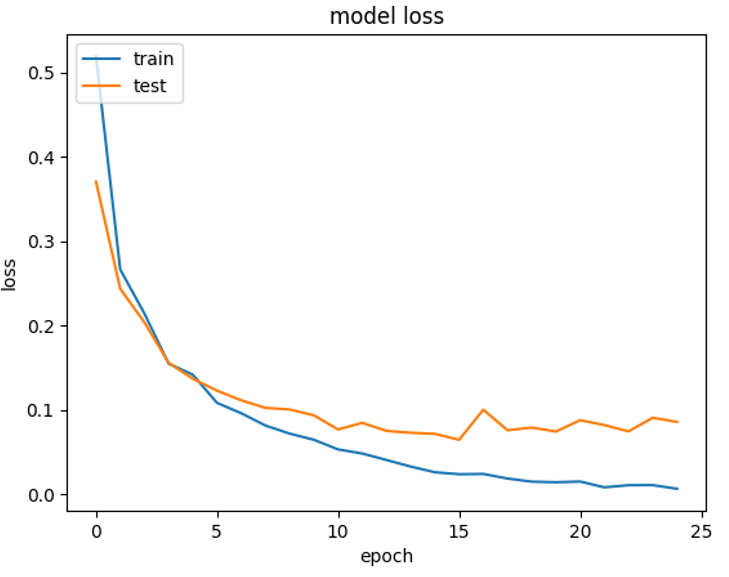
\includegraphics[width=0.5\textwidth]{lossmask.png} &
		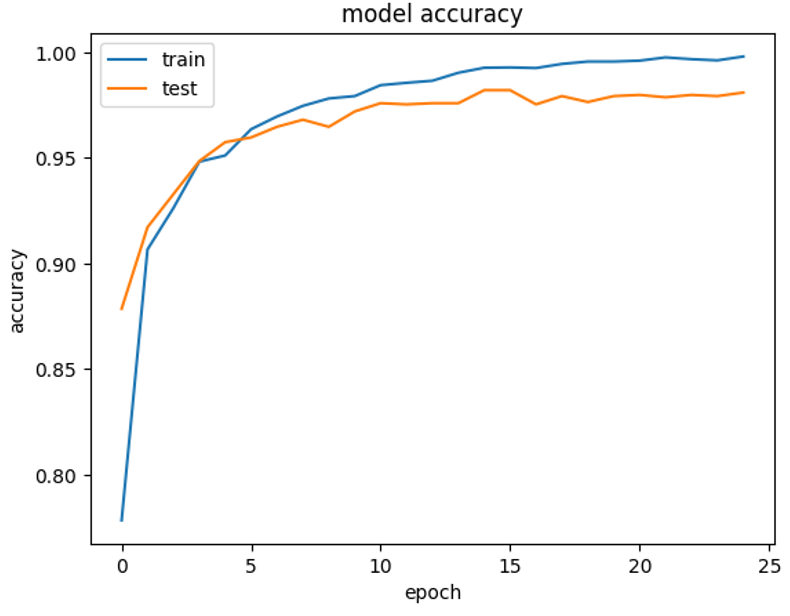
\includegraphics[width=0.5\textwidth]{accmask.png} 
	\end{tabular}
	\caption[Model Accuracy và Model Loss.]{Model Accuracy và Model Loss.}
	\label{fig:modelloss and Model Accuracy}
\end{figure}

Đồ thị ACC,  độ chính xác (Accuracy) lên đến 98\% và bắt đầu ổn định khi epoch = 10,  cho cả tập dữ liệu huấn luyện và tập test, đồ thị Loss của cũng cho thấy sau mức này, Loss của cả tập train và validation. Kết quả cho thấy mô hình có độ phù hợp tốt và không bị quá khớp (over-fitting).

\begin{itemize}
	\item Đánh giá hiệu suất mô hình:

	\begin{figure}[h!]
		\centering
		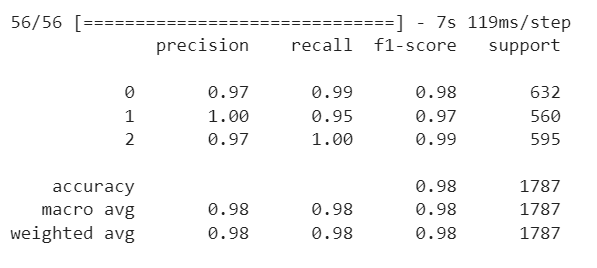
\includegraphics[width=0.6\textwidth]{per.png}
		\caption[Đánh giá hiệu suất mô hình.]{Đánh giá hiệu suất mô hình.}
		\label{fig:per} 
	\end{figure}

	\item Confusion Matrix:
		
	\begin{figure}[h!]
		\centering
		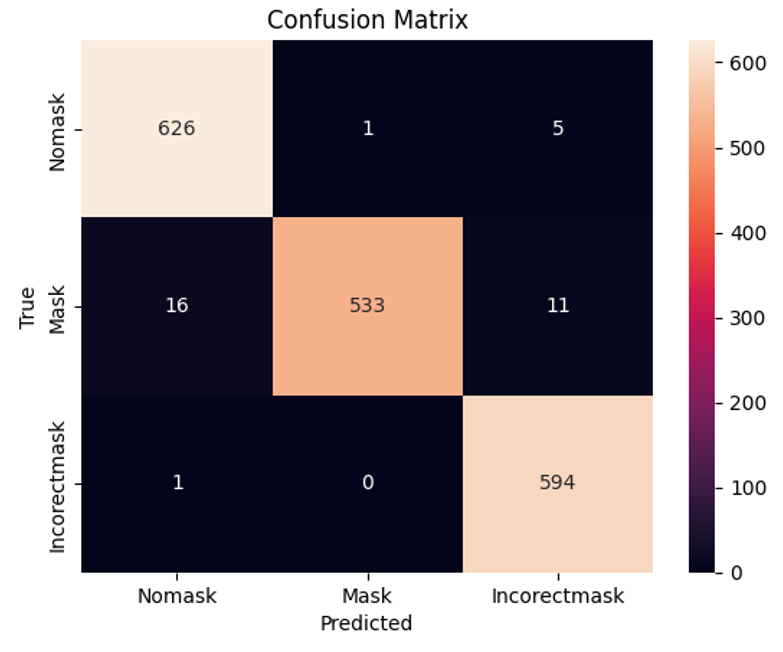
\includegraphics[width=0.53\textwidth]{confu.png}
		\caption[Confusion Matrix.]{Confusion Matrix.}
		\label{fig:confu} 
	\end{figure}
\end{itemize}

\subsubsection{Kết quả huất luyện tập dữ liệu cảm xúc}

\begin{figure}[h!] 
	\begin{tabular}{cc}
		\centering
		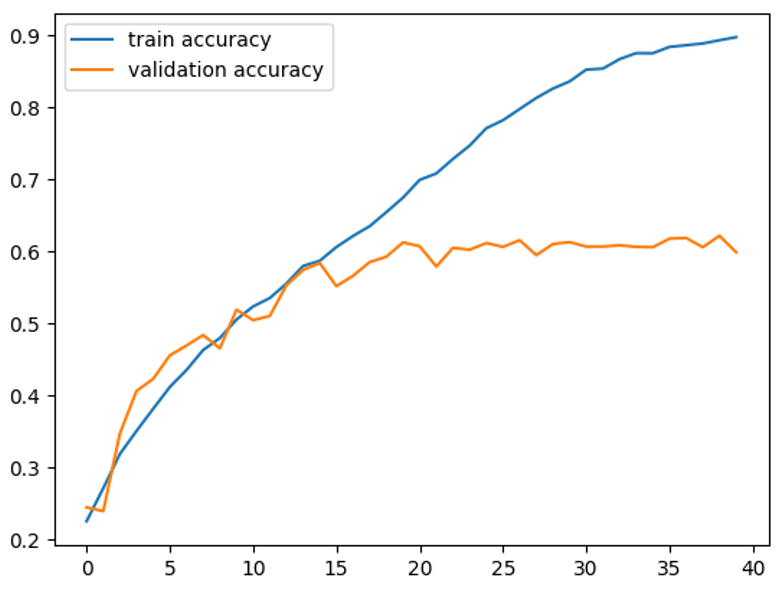
\includegraphics[width=0.5\textwidth]{accemotion.png} &
		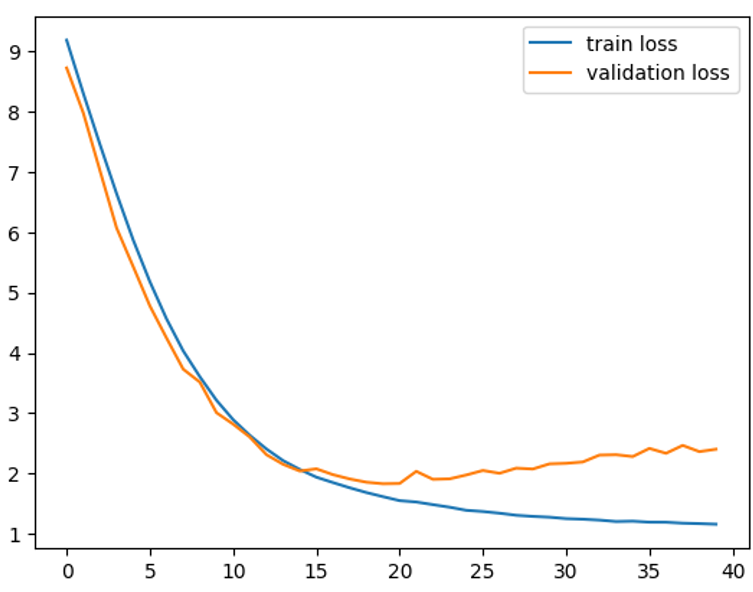
\includegraphics[width=0.5\textwidth]{lossemotion.png} 
	\end{tabular}
	\caption[Model Accuracy và Model Loss.]{Model Accuracy và Model Loss.}
	\label{fig:modelloss_and_Model Accuracy}
\end{figure}

Đồ thị ACC,  độ chính xác (Accuracy) lên đến 98\% ở tập train và 60\% ở tập test và bắt đầu ổn định khi epoch = 20,  cho cả tập dữ liệu huấn luyện và tập test, đồ thị Loss của cũng cho thấy sau mức này, Loss của cả tập train và validation. Kết quả cho thấy mô hình có độ phù hợp tốt và không bị quá khớp (over-fitting).

\begin{itemize}
	\item Đánh giá hiệu suất mô hình:
	
	\begin{figure}[h!]
		\centering
		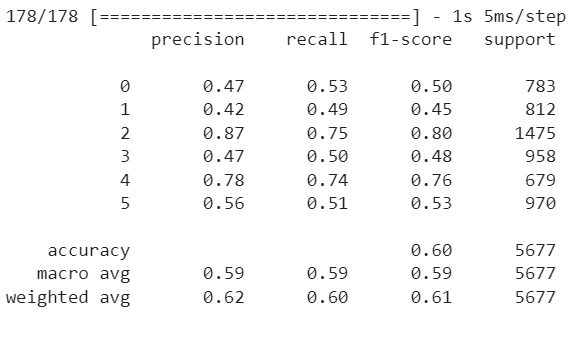
\includegraphics[width=0.7\textwidth]{ac.png}
		\caption[Đánh giá hiệu suất mô hình.]{Đánh giá hiệu suất mô hình.}
		\label{fig:ac} 
	\end{figure}
	
	\item Confusion Matrix:
	
	\begin{figure}[h!]
		\centering
		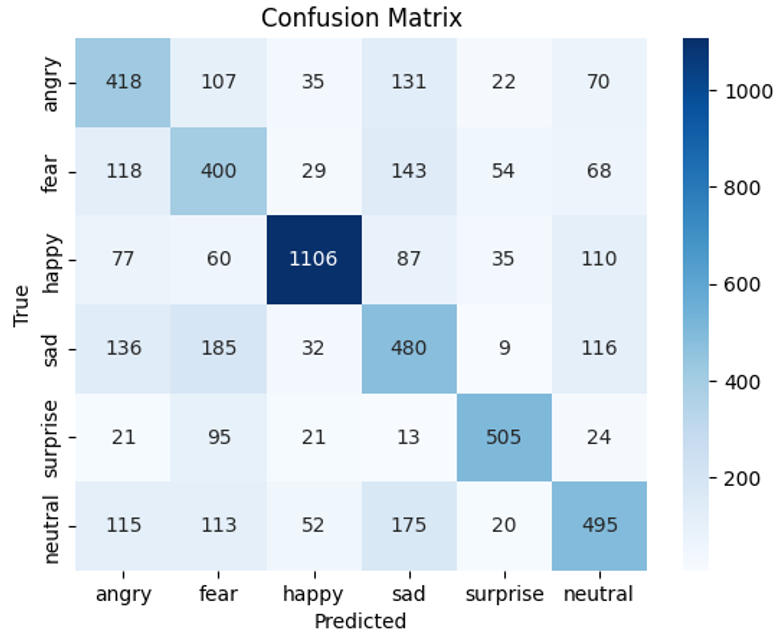
\includegraphics[width=0.6\textwidth]{fu.png}
		\caption[Confusion Matrix.]{Confusion Matrix.}
		\label{fig:fu} 
	\end{figure}
\end{itemize}

\subsection{Thử nghiệm với thời gian thực webcam}

*** Sử dụng thư viện open cv để test kết quả trên thời gian thực 

** Bước 1: Load Model

\begin{lstlisting}[style=codePython]
	from tensorflow.keras.models import load_model
	model1 = load_model('model_mask_final.h5')
	model2 = load_model('model_emotions_final.h5')					
\end{lstlisting}

** Bước 2: Phát hiện khuôn mặt

\begin{lstlisting}[style=codePython]
	prototxt = 'deploy.prototxt'
	model = 'res10_300x300_ssd_iter_140000.caffemodel'
	net = cv2.dnn.readNetFromCaffe(prototxt, model)						
\end{lstlisting}

** Bước 3: Chạy webcam

\begin{lstlisting}[style=codePython]
	cap = cv2.VideoCapture(0)
	
	while True:
	
	ret, frame = cap.read()
	
	if ret:       
		frame = imutils.resize(frame, width=500)
		(h, w) = frame.shape[:2]
		blob = cv2.dnn.blobFromImage(cv2.resize(frame, (300, 300)), 1.0, (300, 300), (104.0, 177.0, 123.0))
		net.setInput(blob)
		detections = net.forward()
		for i in range(0, detections.shape[2]):
			confidence = detections[0, 0, i, 2]
			if confidence > 0.5:
				box = detections[0, 0, i, 3:7] * np.array([w, h, w, h])
				(startX, startY, endX, endY) = box.astype("int")
				y = startY - 10 if startY - 10 > 10 else startY + 10
	
				minX, maxX = min(startX, endX), max(startX, endX)
				minY, maxY = min(startY, endY), max(startY, endY)
				face = frame[minY:maxY, minX:maxX].copy()
				img1 = cv2.resize(face,(48,48))
				img = np.array([img1/255.])
				y_ha = model1.predict(img)
				y_hat = np.argmax(y_ha)
				text= y_ha[0][y_hat]
				text = str(text)
				mask = ('Nomask', 'Mask', 'Incorect')
				predicted_mask = mask[y_hat] 
				cv2.rectangle(frame, (startX, startY), (endX, endY), (0, 0, 255), 2)
				cv2.putText(frame,predicted_mask, (startX, y),cv2.FONT_HERSHEY_SIMPLEX, 0.5, (255, 0, 0), 2) 
				cv2.putText(frame,text, (startX+70, y),cv2.FONT_HERSHEY_SIMPLEX, 0.5, (255, 0, 0), 2) 
				if y_hat ==0:                  
					img = cv2.cvtColor(img1,cv2.COLOR_BGR2GRAY)
					img = np.array([img/255.])
					y_ha2 = model2.predict(img)
					y_hat2 = np.argmax(y_ha2)
					k= y_ha2[0][y_hat2]
					text2 = str(k)
					emotions = ('angry', 'fear', 'happy', 'sad', 'surprise', 'neutral')
					predicted_emotion = emotions[y_hat2]
					cv2.putText(frame,predicted_emotion, (startX,endY+10),cv2.FONT_HERSHEY_SIMPLEX, 0.5, (0,255,0), 2)
					cv2.putText(frame,text2, (startX+70, endY+10),cv2.FONT_HERSHEY_SIMPLEX, 0.5, (255, 0, 0), 2)
	
		cv2.imshow("Detection", frame)
		key = cv2.waitKey(1)
		if key == 27:
			break
	cap.release()
	cv2.destroyAllWindows()							
\end{lstlisting}

**  Bước 4: Demo kết quả chạy webcam

\begin{figure}[h!]
	\centering
	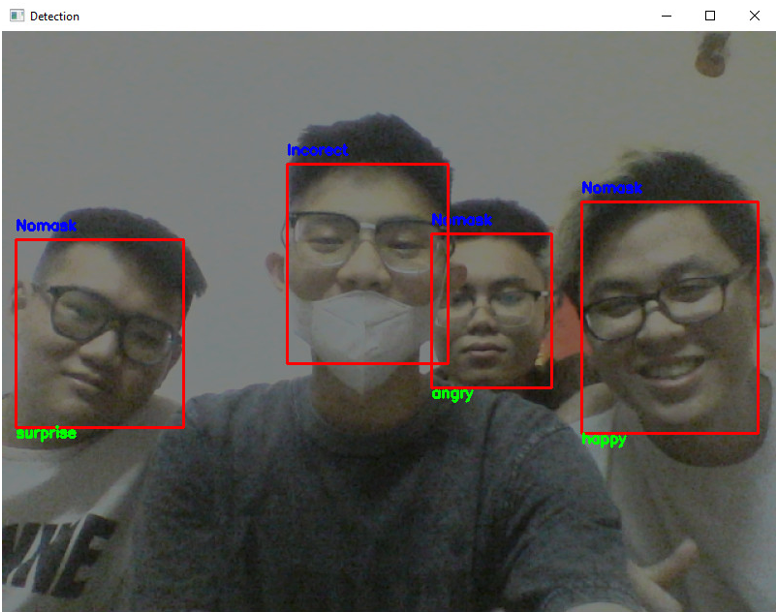
\includegraphics[width=0.6\textwidth]{demo1.png}
	\caption[Demo kết quả chạy webcam1.]{Demo kết quả chạy webcam1.}
	\label{fig:demo1} 
\end{figure}

\begin{figure}[h!]
	\centering
	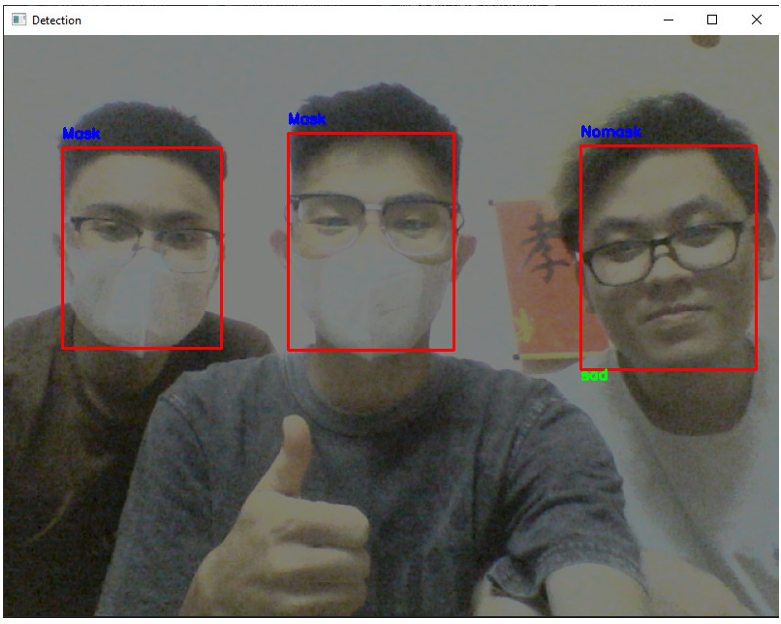
\includegraphics[width=0.7\textwidth]{demo2.png}
	\caption[Demo kết quả chạy webcam2.]{Demo kết quả chạy webcam2.}
	\label{fig:demo2} 
\end{figure}

\begin{figure}[h!] 
	\begin{tabular}{cc}
		\centering
		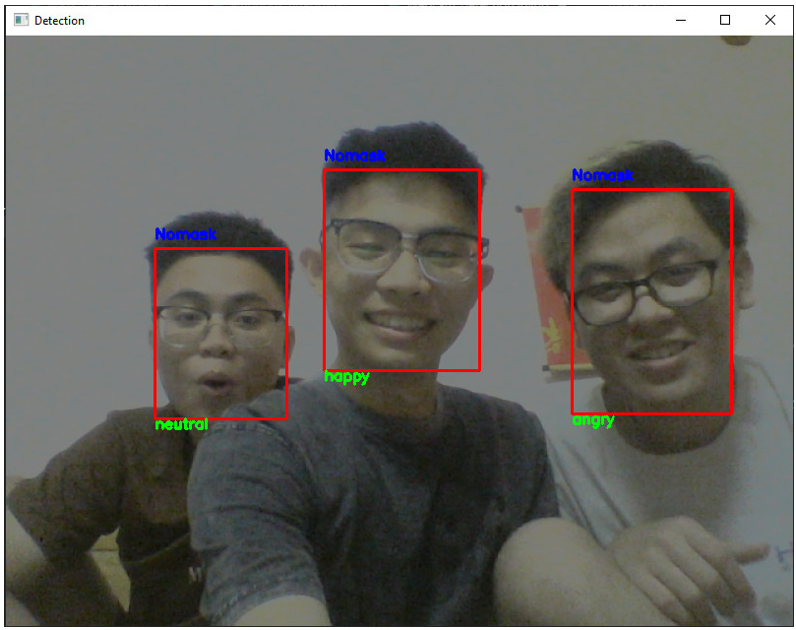
\includegraphics[width=0.5\textwidth]{demo3.png} &
		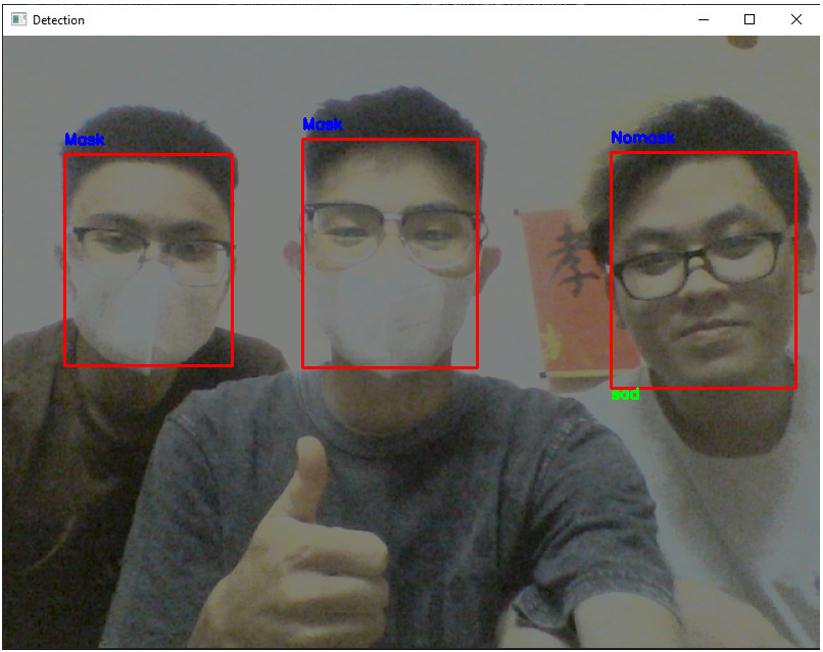
\includegraphics[width=0.5\textwidth]{demo4.png} 
	\end{tabular}
	\caption[Demo kết quả chạy webcam3.]{Demo kết quả chạy webcam3.}
	\label{fig:demo3}
\end{figure}








